%%%%%%%%%%%%%%%%%%%%%%%%%%%%%%%%%%%%%%%%%%%%%%%%%%%%%%%%%%%%%%%%%%%%%%
% AIM 3 PREVIEW -- Yale (Pfaller) contributions to the Research Strategy
%
% Renders the Yale-authored fragments (Innovation subsection, Aim 3
% preliminary-results figure) with the shared project preamble, so they
% appear exactly as they will in grant_application.tex on Overleaf.
% Preview only, not a submission document. \input new Yale fragments
% here as they are drafted.
%%%%%%%%%%%%%%%%%%%%%%%%%%%%%%%%%%%%%%%%%%%%%%%%%%%%%%%%%%%%%%%%%%%%%%
%%%%%%%%%%%%%%%%%%%%%%%%%%%%%%%%%%%%%%%%%%%%%%%%%%%%%%%%%%%%%%%%%%%%%% 
% PREAMBLE
%%%%%%%%%%%%%%%%%%%%%%%%%%%%%%%%%%%%%%%%%%%%%%%%%%%%%%%%%%%%%%%%%%%%%%

% ====================================================================
%       DOCUMENT CLASS
% ====================================================================
\documentclass[11pt,english]{article}


% ====================================================================
%       START PACKAGES, NEW PARAMETERS, AND NEW COMMANDS
% ====================================================================
\makeatletter

% use helvetica as default sans-serif font
\usepackage{helvet}
\renewcommand{\familydefault}{\sfdefault}

% standard font encoding
\usepackage[T1]{fontenc}

% geometry (margins, etc.)
\usepackage[letterpaper]{geometry}
\geometry{verbose, tmargin=0.5in, bmargin=0.5in, lmargin=0.5in, rmargin=0.5in, headheight=0cm, headsep=0cm, footskip=0cm}
\marginparwidth=0pt
\marginparsep=0pt
\pagestyle{empty}
\setcounter{secnumdepth}{4}
\setlength{\parskip}{\smallskipamount}
\setlength{\parindent}{0pt}

% replace underlining in unsrt biblio by emphasis (italic)
\PassOptionsToPackage{normalem}{ulem}

% a bunch of packages
\usepackage{color}
\usepackage{array}
\usepackage{float}
\usepackage{units}
\usepackage{amsbsy}
\usepackage{amssymb}
\usepackage{graphicx}
\usepackage{nccmath}
\usepackage{graphicx}
\usepackage{framed}
\usepackage{setspace}
\usepackage{babel}
\usepackage{textgreek}  % greek letters in the text, no need to use equations
\usepackage{breakcites}
\usepackage{wrapfig}
\usepackage{multirow}
\usepackage{tabularx}
\usepackage{sidecap}
\usepackage{booktabs}
\usepackage{lipsum} % for dummy "lorem ipsum" text
\usepackage[acronym,shortcuts]{glossaries}
\usepackage{subfigure}


% references (use bib file)
\usepackage[superscript]{cite}
\renewcommand{\citeform}[1]{\textbf{#1}}
\renewcommand\@biblabel[1]{[\textbf{#1}] }

% captions
\usepackage{caption}
\DeclareCaptionLabelSeparator{dot}{. }
\captionsetup{labelfont={bf}, font=scriptsize, labelsep=dot}
\useshortskip
\setlength{\floatsep}{0pt}
\setlength{\textfloatsep}{5pt}
\setlength{\abovecaptionskip}{2pt}
\setlength{\belowcaptionskip}{0pt}

% compact titles
\usepackage[compact]{titlesec}
\titlespacing{\section}{0pt}{-1pt}{-1pt}
\titlespacing{\subsection}{0pt}{-1pt}{-1pt}
\titlespacing{\subsubsection}{0pt}{-1pt}{-1pt}

% lists
\usepackage{enumitem}
\setlist{parskip=0pt}
\setlist{leftmargin=*,parsep=1pt,itemsep=2pt,topsep=2pt,partopsep=0pt}
\renewcommand{\labelenumi}{\bfseries\arabic{enumi}.}
\renewcommand{\labelenumii}{\bfseries\alph{enumii}.}

% algorithms
\usepackage{algpseudocode}
\usepackage[plain]{algorithm}  % [options] are [plain], [boxed], [ruled]
\captionsetup[algorithm]{labelfont={bf}, font=scriptsize, labelsep=dot}
\floatstyle{plaintop}
\restylefloat{algorithm}

% colors
\usepackage[svgnames,table]{xcolor}
\definecolor{newgray}{rgb}{0.3882,0.4,0.4157}

% more colors
\usepackage{colortbl}
\definecolor{lightgray}{gray}{0.90}
\definecolor{darkgray}{gray}{0.40}

% new list type (from Lyx)
\newenvironment{lyxlist}[1]
    {\begin{list}{}
        {\settowidth{\labelwidth}{#1}
         \setlength{\leftmargin}{\labelwidth}
         \addtolength{\leftmargin}{\labelsep}
         \renewcommand{\makelabel}[1]{##1\hfil}}}
    {\end{list}}

% arrays setup (for \hline in tables) 
\arrayrulecolor{newgray}
\setlength{\arrayrulewidth}{0.30mm}

% stretch tables row size
\renewcommand{\arraystretch}{1.5}  

\makeatother
% ====================================================================
%       END PACKAGES, NEW PARAMETERS, AND NEW COMMANDS
% ====================================================================

% ====================================================================
%       INPUT LATEX FILES
% ====================================================================
\input{abbreviations}
% Acronym definitions - loaded by definitions.sty
\newacronym{gr}{G\&R}{growth and remodeling}
\newacronym{av}{AV}{atrioventricular}
\newacronym{icmr}{iCMR}{invasive cardiac magnetic resonance}
\newacronym{biv}{BiV}{biventricular}
\newacronym{dt}{DT}{Digital Twin}
\newacronym{hcmm}{hCMM}{homogenized constrained mixture model}
\newacronym{iedv}{iEDV}{indexed end-diastolic volume}

% computational
\newacronym{cfd}{CFD}{computational fluid dynamics}
\newacronym{uq}{UQ}{uncertainty quantification}

% databases
\newacronym{vmr}{VMR}{Vascular Model Repository}

% yale
\newacronym{ycrc}{YCRC}{Yale Center for Research Computing}

% software
\newcommand{\fsi}[0]{{svMultiPhysics}\xspace}
\newcommand{\sv}[0]{{SimVascular}\xspace}
\newcommand{\od}[0]{{svZeroDSolver}\xspace}
\newcommand{\su}[0]{{svSuperEstimator}\xspace}

% in
\newcommand{\invivo}[0]{\textit{in vivo}\xspace}
\newcommand{\invitro}[0]{\textit{in vitro}\xspace}
\newcommand{\insilico}[0]{\textit{in silico}\xspace}
\newcommand{\exvivo}[0]{\textit{ex vivo}\xspace}

\newcommand{\comment}[1]{}
\newcommand{\bfit}[1]{\textbf{\textit{#1}}}
\newcommand{\ulit}[1]{\ul{\textit{#1}}}
\newcommand{\bfulit}[1]{\textbf{\ul{\textit{#1}}}}
\newcommand{\note}[1]{\textbf{\textcolor{red}{#1}}}

% aim block for the Specific Aims page: \aim{number}{title}{body}
% (as in definitions.sty, but without the \\ after the title, which added a blank line)
\usepackage{scrextend}
\newcommand{\aim}[3]{%
\par\textbf{Aim #1: #2}%
\begin{addmargin}[1em]{0em}
#3
\end{addmargin}%
}

\patchcmd{\thebibliography}{\section*{\refname}}{}{}{}

\begin{document}

\note{PREVIEW -- Yale (Pfaller) contributions, rendered with the shared Overleaf preamble.}

% match the counter state of the Innovation subsection in grant_application.tex
\setcounter{section}{1}
\setcounter{subsection}{1}

\subsection{Innovation}

\subsubsection{Predicting Long-Term Ventricular Growth with a Constrained Mixture Model}

Whether a borderline ventricle will grow enough after recruitment to sustain a
biventricular circulation is, at its core, a question of long-term \gls*{gr}: the
myocardium must add mass and reshape its chamber over the 8 to 15 months between
the recruitment procedure and the follow-up exam. No clinical measurement forecasts
this. The suitability criteria in use today, indexed end-diastolic volume and
end-diastolic pressure, describe the ventricle as it is on the day of the exam;
they cannot say whether its tissue will remodel toward an adequate size or stall.
The pre-recruitment \gls*{dt} of Aim~1 captures the ventricle's state, but a snapshot,
however complete, does not contain its trajectory.

\textbf{Growth as a mechanistic process, not a prescribed outcome.} For three decades,
cardiac \gls*{gr} has been modeled almost exclusively with kinematic growth theory,
which imposes the direction and extent of growth through an inelastic growth
tensor. Such models reproduce the shape and mass changes seen in athlete's heart,
dilation, and hypertrophy efficiently, and they have been applied to heart failure
and infarction. But they prescribe the answer rather than predict it: the growth
is put in by hand, decoupled from the tissue-level turnover that actually drives
adaptation, and unable to represent the return to a stable size once loading
normalizes. For a proposal that must decide, before surgery, whether growth will be
\emph{sufficient}, a model whose growth is prescribed cannot provide the answer.

\textbf{A constituent-level model that lets growth emerge.} The constrained mixture
theory instead treats the myocardial wall as a mixture of constituents, contractile
myocytes and passive collagen and matrix, each deposited and degraded to chase a
homeostatic mechanical set-point. Growth is then an emergent consequence of the
imbalance between the tissue's mechanical state and that set-point, exactly the
mechanobiology observed in living myocardium. Our group developed and validated the
first homogenized constrained mixture model of cardiac \gls*{gr}, in which
concentric and eccentric remodeling arise from constituent turnover rather than
being imposed, and which reproduces both stable growth that returns to homeostasis
and unstable growth that runs away, from a single set of equations
(Figure~\ref{fig:aim3prelim}). We subsequently removed the memory barrier that had
confined constrained mixture models to short simulated horizons, making
organ-scale growth over months of physiological time computationally tractable.
These are the two capabilities the recruitment question requires, and both are
already in hand.

\textbf{Why this matters for recruitment.} Recruitment is precisely the setting the
theory was built for: a controlled, sustained change in mechanical load imposed on
a chamber, followed months later by an imaged outcome. Initialized from the
pre-recruitment \gls*{dt} and driven by the post-recruitment loading, the model
predicts the growth trajectory of chamber volume, wall thickness, and mass, and
therefore whether the ventricle reaches an adequate size. A prediction of
\emph{insufficient} growth is the clinically actionable one: it identifies, before
any surgery, the children for whom recruitment would add risk without benefit
before the eventual Fontan, sparing them a futile intermediate operation. This
moves the field beyond size-and-pressure cutoffs toward a mechanistic forecast of
how the individual ventricle will remodel, the long-term counterpart to the
short-term physiology that Aims~1 and~2 recover from the same \gls*{icmr} exam.


\begin{figure}[b!]
    \centering
    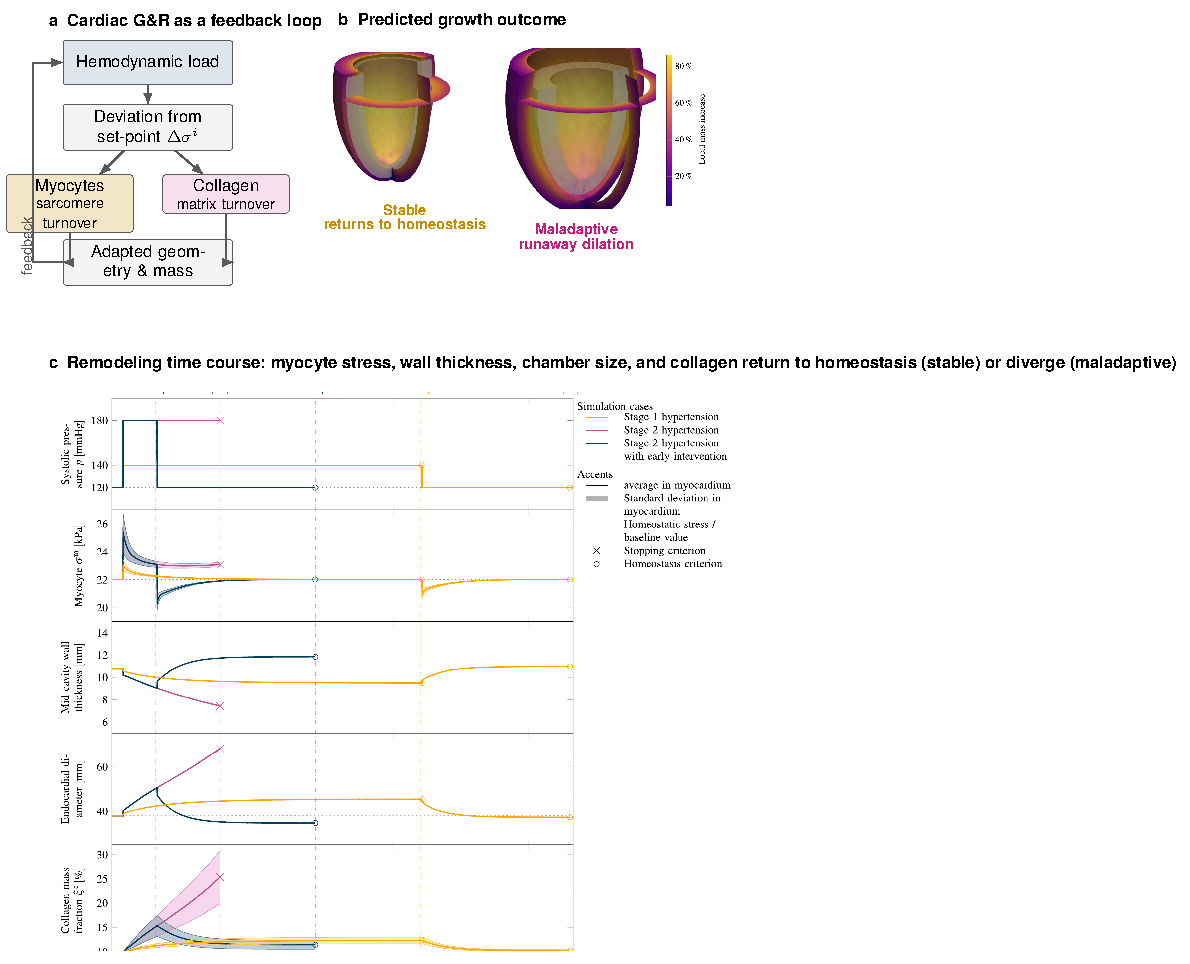
\includegraphics[width=1\linewidth]{figures/aim3_figure.pdf}
    \caption{\textbf{Preliminary results: cardiac \gls*{gr} as a mechanobiological feedback loop.}
    (a)~Constituent-level feedback: deviations of the mechanical state from a homeostatic set-point drive myocyte and collagen turnover, which adapts geometry and mass and feeds back on the load.
    (b)~From a single set of equations, the model predicts both stable growth that returns to homeostasis and maladaptive, runaway dilation.
    (c)~Time courses of myocyte stress, wall thickness, chamber size, and collagen for both outcomes.
    \note{[draft caption -- edit before moving into grant\_application.tex]}}
    \label{fig:aim3prelim}
\end{figure}

\bibliographystyle{mrp}
\bibliography{references,martin_highlighted}

\end{document}
